\chapter{Analiza tematu wyszukiwania tekstu}  % Analiza tematu
% 

%\begin{itemize}
%\item Jaki problem chcę (muszę :-) rozwiązać?
%\item Dlaczego rozwiązanie problemu jest ważne?
%\item Jak inni rozwiązują ten problem?
%\item Jakie są zalety i wady tych rozwiązań?
%\end{itemize}

%Odwołania do literatury:
%książek \cite{bib:ksiazka},
%artykułów w czasopismach \cite{bib:artykul},
%materiałów konferencyjnych \cite{bib:konferencja}
%i stron www \cite{bib:internet}.
%
%Równania powinny być numerowane
\begin{align}
    y = \frac{\partial x}{\partial t}
\end{align}
%
%
%\begin{itemize}
%\item analiza tematu
%\item wprowadzenie do dziedziny (\english{state of the art}) – sformułowanie problemu, 
%\item poszerzone studia literaturowe, przegląd literatury tematu (należy wskazać źródła wszystkich informacji zawartych w pracy)
%\item opis znanych rozwiązań, algorytmów, osadzenie pracy w kontekście
%\item Tytuł rozdziału jest często zbliżony do tematu pracy. 
%\item Rozdział jest wysycony cytowaniami do literatury \cite{bib:artykul,bib:ksiazka,bib:konferencja}. 
%Cytowanie książki \cite{bib:ksiazka}, artykułu w czasopiśmie \cite{bib:artykul}, artykułu konferencyjnego \cite{bib:konferencja} lub strony internetowej \cite{bib:internet}.
%\end{itemize}

\begin{Definition}\label{def:1}
Definicja to zdanie (lub układ zdań) odpowiadające na pytanie o strukturze „co to jest a?”. Definicja normalna jest zdaniem złożonym z 2 członów: definiowanego (łac. definiendum) i definiującego (łac. definiens), połączonych spójnikiem definicyjnym („jest to”, „to tyle, co” itp.). 
\end{Definition}

\begin{Theorem}[Pitagorasa]\label{t:pitagoras}
W dowolnym trójkącie prostokątnym suma kwadratów długości przyprostokątnych jest równa kwadratowi długości przeciwprostokątnej tego trójkąta. 
\end{Theorem}

\begin{Example}[generalizacja]\label{ex:generalizacja}
Przykładem generalizacji jest para: zwierzę i pies. Pies jest zwierzęciem. Pies jest uszczegółowieniem pojęcia zwierzę. Zwierzę jest uogólnieniem pojęcia pies.
\end{Example}
\section{Sformułowanie problemu}
Wyszukiwanie tekstu w systemach towarzszy ludziom od początków istnienia maszyn,
choć pierwsze komputery nie posiadały ogromnych ilość pamięci co nie powodowało
potrzeby istnienia algorytmów wyszukujących tekst. Procesor Intel 8008 
zaprezentowany w 1972 posiadał jedynie 14 bitową magistrale adresową co 
pozwalało na 16 Kbi pamięci. Model Motoroli 68000 posiada 5 MB dysku twardego,
co nie może się równać z opecnym standardem darmowej pamięci udostępnianej w 
chmurze przez Google (15 GB).

Zasadniczym problem naszej pracy jest wyszukiwanie zawartości tekstowej
ogramnej ilość plików w różnych formatach. Takie podejście może okazać się 
problematyczne w przypadku plików dzwiękowych, filomowych czy zdjęć wszelkiego
rodzaju.

\section{State of art}

Podjęcie problemu wyszukiwania plików po nazwach oraz zawartości jest bardzo
złożonym i trudnym problemem w sferze programistycznej. Istnieje wiele rozwiązań
tego problemu, które istnieją od początku pracy z komputerem. Narzędzia takie
jak \textbf{find}, \textbf{grep} czy \textbf{fzf} \cite{bib:internet:Fzf} pozwalają na wyszukiwanie
zawartości która nas interesuje, ale kompleksowość tych narzędzi nie jest 
przystosowana do tak trudnego problemu, jakim jest wyszukiwanie treści w plikach,
które są zarchiwizowane. Z taką samą niedogodnością spotykamy się w przypadku
plików pochodzących z pakietu Microsoft Office 365, jednak jeśli rozwiążemy 
zadanie otrzymywania zawartości z archiwów, będziemy w stanie otrzymać również 
zawartość z plików z rozszerzeniami .doc, .docx czy .pptx.

\subsection{Przykładowe narzędzia dostępne do wykorzystania}

Narzędzie \textbf{find} to znane i popularne narzędzie wśród osób zaznajomionych z
technologiami linuxowymi. Już bardzo często wykorzystywany do znajdowania plików
w systemie, jednak nie nadaje sie do znajdowania zawartości plików.

Przykłady użycia programu find:
\begin{itemize} 
  \label{fig:find-example}
  \item find rootPath -name '*.ext'
  \item find rootPath -path 'path/*.ext' 
  \item find rootPath -name '*.py' -not -path '*/site-packages/*'
  \item find rootPath -maxdepth 1 -size +500k -size -10M
  \item find rootPath -type f -empty -delete
\end{itemize}
%\begin{figure}[h]
%  \centering
%  \begin{lstlisting}
%  \end{lstlisting}
%  \caption{Przykłady użycia programu find}
%  \label{fig:code:bashFindExamples}
%\end{figure}

Do przeszukiwania zawartości plików dobrze nadaje się narzędzie grep, który jest
dostępny w każdej dystrybucji Linuxa. Jego działanie jest dość podobne do finda,
lecz posiada on możliwość wyszukiwania treść w plikach tekstowych, lecz nie w 
archiwach. Grep nie posiada też możliwość szukania zawartości plików .pdf oraz
nie wspiera formatów książkowych takich jak .djvu.

Przykłady użycia programu find:
\begin{itemize} 
  \label{fig:grep-example}
  \item grep "searchPattern" path/to/file
  \item grep -F|--fixed-strings "exactString" path/to/file
  \item cat path/to/file | grep -v|--invert-match "searchPattern"
\end{itemize}

Istnieje również ripgrep, który jest sukcesorem wcześniej wymienionego
narzędzia. Jego wydajność przewyższa grepa nawet trzydziestokrotnie w niektórych
testach sprawnościowych, jednak zazwyczaj jest to niewielki wzrost. Nie jest on
niestety domyślnie instalowany na większości systemów linuxowych. Nie posiada on
również wsparcia dla formatów pdf i djvu.

Można wyszukiwać również po treści piosenek, ale wymagałoby to utworzenie modelu
sztucznej inteligencji, która wydobywałaby tekst z piosenek do postaci tekstowej.

\section{Odniesienia do literatury}

Istnieje wiele odniesień do wyszukiwania danych w literaturze. Praca Google 
\cite{bib:internet:htmlSearchGoogle} odnosi się do problemu wyszukiwania tekstu 
w dobie internetu i ilości danych, która jest przechowywana w chmurze. Wymagane
jest indeksowanie, które przyspiesza wyszukiwanie, ale wykonane nie poprawnie 
skutkuje słabymi wyszukiwaniami. Ilość danych wydobywana i dostarczana do
użytkowników stanowi duże wyzwanie oraz wymaga wykorzystania skomplikowanych 
algorytmów. 

Należy również mieć świadomość, że wyszukiwanie tekstu html posiada dodatkową 
złożoność związaną z linkami (ang. \english{anchor}). Linki mogą prowadzić do 
kolejnych stron lub plików, które należy przeszukać w celu wydobycia informacji.
Powoduje to, że proste wyszukiwanie wymaga adaptacji kodu, aby odnieść się do 
przypadków o których wcześniej nie wiedziano.

W plikach, które znajdują się na stronach mogą być na przykład archiwa, które
mają różne wielkości oraz różne typy kompresji. Dodatkowo kompresja może być 
bardziej agresywna lub nawet stratna.

Podczas konferencji TREC \cite{bib:konferencja:TRECDuplicates} jeden z zespołów 
napotkał problem, duplikacji danych. Chęć wydobycia danych w celu utworzenia
tekstów wymagało odpowiedniej deduplikacji dokumentów oraz wyborze tej treści,
która posiada najwięcej wartości. Mogłoby to być tematem rozszerzenie pracy. 

\textbf{TODO MORE PAPERS ADDED}

\section{Opis poznanych rozwiązań}
\subsection{Algorytm brute force}

Jest wiele algorytmów, które wyszukują tekst. Jednym z takich algorytmów jest 
algorytm typu brute-force. Polega sprawdzaniu każdego bajtu, jego implementacja
jest bardzo prosta i standardowa, a złożoność czasowe tego rozwiązania wynosi
O(m * n), gdzie m to długość bloku (pattern), a n to długość tekstu (substring),
którego szukamy. 

\begin{figure}[h]
  \centering
  \begin{lstlisting}
for i := 0; i<len(pattern); i++{
  for j := 0; j<len(substring); j++{
    // compare bytes
  }
}
  \end{lstlisting}
  \caption{Przykłady algorytmu brute force}
  \label{fig:code:bruteForceComparison}
\end{figure}

Zaletą tego algorytmu jest to, że nie posiada potrzeby przechowywać żadnych 
danych w pamięci. Ten algorytm dobrze sprawdza się gdy posiadamy ograniczoną 
ilość zasobów pamięci, co nie jest problemem w obecnych czasach, gdy pamięć jest
stosunkowo tania i szeroko dostępna.
\begin{figure}[h]
  \centering
  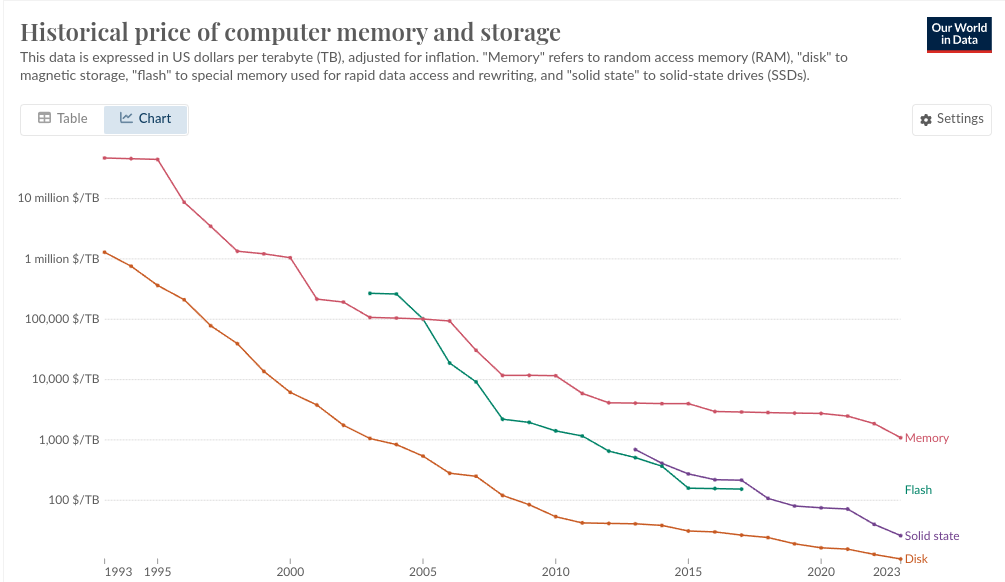
\includegraphics[width=0.9\textwidth]{./images/historical-mem-price.png}
  \caption{Historyczne dane cen pamięci w latach 1993-2023 }
  \label{screenshot:MemPrices}
\end{figure}
%\cite{internet:HistoricalMemPrice}
%https://jcmit.net/memoryprice.htm

Powyższy algorytm można zrównoleglić, dzieląc wzorzec na mniejsze części
i wyszukując tylko dane w tym obszarze, ale należy dołożyć końce wzorca, aby nie
wynikła sytuacja, w której wzorzec by wystąpił, ale nie wzięto pod uwagę końca 
zdania. 

\begin{center}
  \begin{tabular}{ |c|c|  } 
    \hline
    \multicolumn{2}{|c|}{TYTUL} \\
    \hline
    wzorzec & ABCABCABDABD \\
    \hline
    podłańcuch & BCA \\
    \hline
    rezultat & 4 \\
    \hline
  \end{tabular}
\end{center}

Jeżeli podzielimy wzorzec na dwa procesy wyszukujące algorytmem brute-force,
otrzymamy dwa zadania:

\begin{center}
  \begin{tabular}{ |c|c||c|c|  } 
    \hline
    \multicolumn{4}{|c|}{Zadania} \\
    \hline
    Zadanie 1 & & Zadanie 2 & \\
    \hline
    wzorzec & ABCABC & wzorzec & ABDABD \\
    \hline
    podłańcuch & BCA & podłańcuch & BCA \\
    \hline
    rezultat & -1 & rezultat & -1 \\ 
    \hline
  \end{tabular}
\end{center}

Zrównoleglenie procesu powoduje, że otrzymaliśmy nie poprawny wynik, gdyż w 
żadnym z wzorców nie występuje podłańcuch "BCA", choć łańcuch występuje w 
miejscu 4, to algorytm nie posiada wiedzy o dalszej części wzorca.

Aby poprawić dany algorytm należy dołożyć znaki, które należy sprawdzać w 
przypadku poprawnego rozpatrzenia ostatniego znaku.


\begin{center}
  \begin{tabular}{ |c|c||c|c|  } 
    \hline
    \multicolumn{4}{|c|}{Zadania} \\
    \hline
    Zadanie 1 & & Zadanie 2 & \\
    \hline
    wzorzec & ABCABC(AB) & wzorzec & ABDABD(nil) \\
    \hline
    podłańcuch & BCA & podłańcuch & BCA \\
    \hline
    rezultat & 4 & rezultat & -1 \\ 
    \hline
  \end{tabular}
\end{center}

W takim przypadku sprawdzamy tylko do sytuacji, w której BC jest częścią
podłańcucha, ale podłańcuch nie został w pełni znaleziony. Długość ponownego 
wyszukania byłaby równa len(podłańcuch) - 1.

\subsection{Algorytm Morisa-Pratta}

Algorytm Morisa-Pratta jest dość prostym algorytmem wykorzystującym możliwość
wcześniejszego sprocesowania podłańcucha wyszukiwanego w tekście co przyspiesza
sposób procesowania tekstu. Polega on na wykorzystaniu faktu istnienia pasującego
prefikso sufiksu. Pozwala to na pominięcie pewnych porównania niektórych znaków,
bez szkody w wyniku wyszukiwania.

Dzięki wykorzystaniu tej zależności możemy uniknąć cofania się indeksu i. 
Tablice preproc wypełniamy poprzednią wartości tak długo aż zaistnieje różnica 
pomiędzy obecnym a następnym znakiem tablicy substr. W przypadku różnicy 
zwiększamy wartość zapisywaną do tablicy preprocesora o odległość różnicy znaków.
W ten sposób następnym razem będzie możliwość pominięcia porównania tych znaków.

\begin{figure}[h]
  \centering
  \begin{lstlisting}
curr = -1
preproc[0] = -1
for i := 1; i <= len(substr); i++ {
  for (curr > -1) && (substr[curr] != substr[i-1]) {
    curr = preproc[curr]
  }
  curr++
  preproc[i] = curr
}
  \end{lstlisting}
  \caption{Przykład preprocesowania podłańcucha }
  \label{fig:code:preprocessMorisPratt}
\end{figure}

W drugim etapie można wykorzystać wcześniej przygotowaną tablice przemieszczeń 
\textbf{preproc}, aby obliczyć ilość przesunięcia w przypadku znalezienia 
niepasującego prefiksu. Dzięki temu zwykle dłuższy tekst znajdujący się w 
\textbf{s} możemy przeanalizować szybciej niż w przypadku algorytmu bruteforce.
Powoduje to niestety problem w przypadku, gdy napis w którym wyszukujemy nie 
jest wystarczająco długi.

\begin{figure}[h]
  \centering
  \begin{lstlisting}
res := []int{}
curr := 0
found := 0
for i := 0; i < len(s); i++ {
  for (curr > -1) && (substr[curr] != s[i]) {
    curr = preproc[curr]
  }
  curr++
  if curr == len(substr) {
    for found < i-curr+1 {
      found++
    }
    res = append(res, found)
    found++
    curr = preproc[curr]
  }
}
  \end{lstlisting}
  \caption{Przykład preprocesowania podłańcucha }
  \label{fig:code:preprocessMorisPratt}
\end{figure}

W podstawowej bibliotece języka Golang, w pakiecie \textit{strings} istnieje 
implementacja metody \textit{Index()}. Nie jest ona jednak w pełni przedstawiona
w kodzie, natomiast w jej implementacji można zauważyć, że algorytm brute force
jest wykorzystywany tylko w przypadku gdy długość wzorca wynosi więcej niż 64.

\begin{figure}[h]
  \centering
  \begin{lstlisting}
func Index(s, substr string) int {
  n := len(substr)
	switch {
	case n == 0:
		return 0
  [...]
	case n > len(s):
		return -1
	case n <= bytealg.MaxLen: // Zwykle ten case
		// Use brute force when s and substr both are small
		if len(s) <= bytealg.MaxBruteForce /* 64 */{
			return bytealg.IndexString(s, substr)
		}
  [...]
  }
}
  \end{lstlisting}
  \caption{ Szukanie łańcucha w standardowej bibliotece Golang }
  \label{fig:code:preprocessMorisPratt}
\end{figure}

W przypadku w go gdy wzorzec jest większy niż 64 to wykonuje się algorytm 
podobny do Morisa-Pratta, który jednak posiada dodatkową walidacje w przypadku
odkrycia false positives. Algorytm Morisa-Pratta nie potrzebuje takiej walidacji.
